%
% Method
%

% !TEX root = ../../main.tex

\chapter{Methode}

  \todo[inline]{Beschreibt die Grundüberlegungen der realisierten Lösung (Konstruktion/Entwurf) und die
  Realisierung als Simulation, als Prototyp oder als Software-Komponente}
  \todo[inline]{Definiert Messgrössen, beschreibt Mess- oder Versuchsaufbau, beschreibt und dokumentiert
  Durchführung der Messungen/Versuche}
  \todo[inline]{Experimente}
  \todo[inline]{Lösungsweg}
  \todo[inline]{Modell}
  \todo[inline]{Tests und Validation}
  \todo[inline]{Theoretische Herleitung der Lösung}

  \section{Design der Individuen}

    \subsection{Körper\label{sub:Körper}}

      Die erste Frage welche sich stellt ist wie kann der Körper am besten beschrieben werden?
      \\
      Der Körper setzt sich aus verschiedenen Punkten auseinander.
      Die mindest- Anzahl solcher Punkte wird auf 4 in einem ersten Schritt festgelegt.
      \\
      Die Obergrenze bei 8.
      Dies gibt dem Körper eine polygon-artige Figur.

      \subsubsection{Hypothese Körperpunkte\label{subsub:hypoKp}}

        Es wird die Hypothese aufgestellt,
        dass sich ein Individuum mit 8 Körperpunkten schneller durch den Parcours bewegen kann,
        als ein Individuum mit weniger Körperpunkten.
        Die Vermutung dabei ist, dass durch die komplexere Form des Individuums,
        die Balance besser gehalten werden kann.
        Ob dies zutrifft wird im Kapitel~\ref{chap:Resulate} diskutiert.

    \subsection{Beine\label{sub:Beine}}

      Insgesamt weissen die Individuen 6 Beine auf. Ein Beinpaar ist symmetrisch. Ein Bein hat jeweils 2 Gelenke,
      eines welches es mit dem Körper verbindet,
      das andere welches Ober- mit Unterschenkel verbindet.
      Als Vereinfachung wird die Höhe des Gelenkes 0 gesetzt  \(h_{a} = 0\)
      Das Bein weisst eine Höhe \(h_{l}\) auf. Die Gelenke verbinden jeweils den Körper mit dem Gelenk und Ober- mit
      Unterschenkel. Es wird ein Höhenfaktor \(hf\) bestimmt, welcher die Höhe des Unterschenkels definiert.
      Die Breite des Beines wird mit \(w_{l}\) bezeichnet.
      \\
      \begin{figure}[H]
        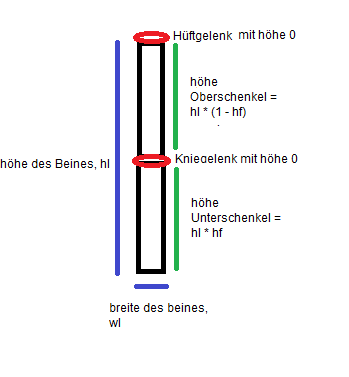
\includegraphics[scale=1]{graphics/leg}
        \caption{Konzept Bein\label{fig:conceptLeg}}
      \end{figure}

      \subsubsection{Masse\label{subs:Masse}}

        Das ganze Individuum weisst eine fixe Masse von 1 auf \(m = 0\).
        Die Masse wird anhand der Fläche der einzelnen Körperteile aufgeteilt.
      \paragraph{Beispiel\label{par:MasseExample}}
        Wenn die Fläche des Körpers Zwei Einheiten gross ist und die Beine jeweils eine Einheit,
        erfolgt folgende Berechnung:
        \\
        \\
        \(m = 1\) \\
        \(A_{Bein} = 1\) \\
        \(A_{Körper} = 2\) \\
        \(A_{total} = A_{Bein} * 6 + A_{Körper} = 8 \) \\
        \( x = m / A_{total} = 0.125 \) \\
        \(m_{Bein} = x * A_{Bein} = 0.125\) \\
        \(m_{Körper} = x * A_{Körper} = 0.25\) \\

    \subsection{Genotyp\label{sub:Genotype}}

      \subsubsection{Design\label{subsub:GenotypeDesign}}

        Der Anspruch an das Design des Genotyps ist möglichst modular und einfach zu sein.
        Als Grund für ein modulares Design spricht die Erweiterbarkeit und Wiederverwendung der bestehenden Teile.
        Deshalb wurde der Genotyp in Teil-Genotypen unterteilt.
        Ein Teil-Genotyp repräsentiert dabei eine beliebige Eigenschaft des Individuums.
        Weiter können Teil-Genotypen wiederum in verschiedene weitere Teile aufgespalten werden.
        Damit entsteht die Möglichkeit Individuen nach einem dynamisch generierten Bauplan zu erstellen
        und beliebige Kombinationen aus vorhandenen Teil-Genotypen innerhalb eines Genotyps zu bilden,
        ohne dass die Implementation der seed-Funktion angepasst werden muss.

        \subsubsection{Seeding\label{subsub:GenotypeSeeding}}

          Die initiale Population wird zufällig erstellt. Dieser Vorgang wird Seeding genannt.
          Dabei wird eine Anzahl von Individuen zufällig generiert.
          Unter gewissen Umständen ist es jedoch hilfreich gewisse Parameter nicht zufällig generieren zu lassen
          sondern mit einem fixen Wert zu initialisieren.
          Besonders der Bewegungsablauf kann so von Beginn an festgelegt werden.
          Deshalb wurde beim Seeding ein Ansatz gewählt, der es erlaubt flexibel jeden Teil-Genotyp separat mit
          spezifizierten Werten zu initialisieren.

      \subsubsection{Generierung Körperpunkte\label{subsub:GenotypGenerierungKörperpunkte}}

        Es werden Körper mit 4--8 Punkten generiert. Dazu wird der Einheitskreis in 4--8 Sektoren unterteilt
        Der Winkel eines Sektors entspricht \(\pi / Anzahl Punkte\).
        \\
        Anschliessend wird in jedem Kreissektor mit Hilfe von Polar Koordinaten ein Punkt bestimmt.
        \\
        \( r = random (0, 1), winkel = random(startSektorWinkel, endeSektorWinkel ) \)
        Anschliessend werden die Polarkoordinaten in kartesische Koordinaten transformiert.
        Die Punkte verbunden, ergeben den Körper des Individuum.
        \\
        Zuerst wurde ein Ansatz mit einem Quadrat evaluiert, bei diesem stellte sich jedoch die zufällige Bestimmung
        der Punkte als viel schwerer als mit einem Einheitskreis heraus. Der Nachteil unserer gewählten
        Ansatzes ist, dass eine quadratische Form nur angenähert werden kann.
        Die folgende Abbildung~\ref{fig:kp} zeigt die Punkte eines Individuum mit 6 Körperpunkten:
        \\
        \begin{figure}[H]
          % !TEX root = ../main.tex

\begin{tikzpicture}[scale=5.3,cap=round,>=latex]
 % draw the coordinates
 \draw[->] (-1.5cm,0cm) -- (1.5cm,0cm) node[right,fill=white] {$x$};
 \draw[->] (0cm,-1.5cm) -- (0cm,1.5cm) node[above,fill=white] {$y$};

 % draw the unit circle
 \draw[thick] (0cm,0cm) circle(1cm);

 \foreach \x in {0,60,...,360} {
         % lines from center to point
         \draw[black] (0cm,0cm) -- (\x:1cm);
         % dots at each point
         \filldraw[black] (\x:1cm) circle(0.4pt);
         % draw each angle in degrees
         \draw (\x:0.6cm) node[fill=white] {};
 }

 \foreach \x in {30} {
         % dots at each point
         \filldraw[red] (\x:0.4cm) circle(0.4pt);
         \draw (\x:0.5cm) node[fill=white] {\(P_{0}\)};

 }

 \foreach \x in {110} {
         % dots at each point
         \filldraw[red] (\x:0.4cm) circle(0.4pt);
         \draw (\x:0.5cm) node[fill=white] {\(P_{1}\)};

 }

 \foreach \x in {150} {
         % dots at each point
         \filldraw[red] (\x:0.8cm) circle(0.4pt);
         \draw (\x:0.9cm) node[fill=white] {\(P_{2}\)};
 }

 \foreach \x in {220} {
         % dots at each point
         \filldraw[red] (\x:0.3cm) circle(0.4pt);
         \draw (\x:0.4cm) node[fill=white] {\(P_{3}\)};


 }

 \foreach \x in {280} {
         % dots at each point
         \filldraw[red] (\x:0.6cm) circle(0.4pt);
         \draw (\x:0.7cm) node[fill=white] {\(P_{4}\)};


 }

 \foreach \x in {340} {
         % dots at each point
         \filldraw[red] (\x:0.2cm) circle(0.4pt);
         \draw (\x:0.3cm) node[fill=white] {\(P_{5}\)};

 }

 % draw each angle in radians
 \foreach \x/\xtext in {
     60/\frac{\pi}{3},
     120/\frac{2\pi}{3},
     180/\pi,
     240/\frac{4\pi}{3},
     300/\frac{5\pi}{3},
     360/2\pi}
         \draw (\x:0.85cm) node[fill=white] {$\xtext$};



 % draw the horizontal and vertical coordinates
 % the placement is better this way
 \draw (-1.25cm,0cm) node[above=1pt] {$(-1,0)$}
       (1.25cm,0cm)  node[above=1pt] {$(1,0)$}
       (0cm,-1.25cm) node[fill=white] {$(0,-1)$}
       (0cm,1.25cm)  node[fill=white] {$(0,1)$};
\end{tikzpicture}

          \caption{Berechnung Körperpunkt veranschaulicht\label{fig:kp}}
        \end{figure}

  \subsection{Phenotyp\label{sub:Phenotyp}}

    Der Phenotyp stell die Repräsentation des Genotyps in der Physik Engine dar.
    Er setzt sich aus mehreren geometrischen Figuren zusammen. Die Beine des Individuums
    werden mit Hilfe eines sogenannten Revolute Contraint an den Körper gebunden.
    Ebenso wird der Ober- mit dem Unterschenkel mit solch einem Constraint verbunden.
    Auf allen Revolute Contraint wird ein Rotationsmotor für die Bewegung definiert.

  \subsection{Engine\label{sub:Engine}}

    Die Bewegungs-Engine kontrolliert die Bewegung eines Phenotyps
    Konkreter werden die Hüft- und Knie-Gelenke und deren Motoren kontrolliert.
    Dabei definiert eine Bewegung z.B. wann ein Winkel eines Gelenkes gehalten werden muss
    oder wann der Motor des Gelenkes in welche Richtung in Bewegung gesetzt werden soll.
    \\
    Der Zustand des Bewegungsablaufs wird auf dem Phenotyp festgehalten.
    Es wird gespeichert welche die aktuelle Bewegung ist.
    Die Implementation der Bewegungs-Engine ist eine Finite State Machine (FSM),
    die in gewissen Zuständen stehen bleiben kann.
    \\
    Jedes Individuum verfügt über einen eigenen Bewegungsablauf.
    Der Bewegungsablauf ist eine Liste von parametrisierten Bewegungen
    Dieser wird in die Bewegungs-Engine eingespeist.

    % TODO

    \subsubsection{Bewegung\label{subsub:EngineMovement}}

      Eine Bewegung ist ein Zustand der Bewegungs-Engine.
      Sie legt fest, wann zum nächsten Zustand gewechselt werden kann.
      Unter einer Bewegung wird das Setzten der maximalen und minimalen Winkel oder auch
      das Warten auf einen Zustand eines Gelenkes verstanden.

  \subsection{Notwendige Zusätzliche Implementierungen}

    Die Physik Engine enthält mehrere Fehler, deren Korrektur ist nicht die Aufgabe dieser Bachelorarbeit.
    Für die Erstellung des Terrains wird ein Höhenfeld von p2.js benutzt.
    Die Kollisionserkennung scheint wenig ausgereift zu sein
    zwischen einem Polygon und dem Höhenfeld. Das hat zur Folge, dass die Individuen häufig im Boden versinken.
    Das Problem kann teilweise umgangen werden, in dem kleine Kreise an die Ecken des Körpers jeweils gesetzt werden.
    Kreise wurden auch an die Eckpunkte der Beinteile gesetzt,
    da die Physik Engine ebenfalls Schwierigkeiten hat die Kollision
    zwischen einem Rechteck und einem Höhenfeld zu erkennen.

  \section{Auswahl des Evolutionären Algorithmus}

    Es stehen 4 Typen von Evolutionäre Algorithmen zur Auswahl:
    \begin{itemize}
      \item Genetische Programmierung~\ref{item:genProg}
      \item Genetischer Algorithmus~\ref{item:genAlgo}
      \item Evolutionäre Strategie~\ref{item:evStart}
      \item Evolutionäre Programmierung~\ref{item:evProg}
    \end{itemize}
    \todo[inline]{Genauer Ausführen warum}
    Um die Problemstellung zu lösen, wurde entschieden Evolutionäre Programmierung einzusetzen
    Warum Evolutionäre Programmierung eingesetzt wird, wird nachfolgend erläutert.
    Das Austauschen der Genen, Rekombination, macht keinen Sinn wenn man Individuen das Laufen beibringt.
    Man stelle sich dazu vor, man tausche das Gen welches den Körper definiert, mit dem der Beine.
    Dies stellt schon den ersten Indikator dafür da,
    dass Evolutionäre Programmierung eingesetzt werden kann. Ein weiteres Kriterium ist die genetische Repräsentation.
    Da unser Individuum sich aus Punkten im einem Koordinatensystem,
    verschiedene Winkel und einem Antrieb (Motor) definiert, wird die reale Werte Repräsentation eingesetzt.
    Eine Baumrepräsentation oder binäre Repräsentation erscheint hier wenig gewinnbringend.
    Ein Punkt ist nichts anderes als zwei reale Werte,
    ein Winkel kann ebenfalls so beschrieben werden und ein Antrieb auch.
    Die Problemstellung würde wahrscheinlich anders bewältigt werden,
    würde es hier um reale Kreaturen gehen und nicht nur um virtuelle Roboter,
    welche in einer künstlichen Umgebung (virtuelles Koordinatensystem) das Laufen lernen.

  \section{Eingesetzte Technologien\label{sec:Technology}}

    Zur Auswahl standen mehrere Programmiersprachen und Physik Engines.
    Die Evaluationskriterien dabei waren:
    \begin{itemize}
      \item Platform-Interoperabilität (Linux, Windows Mac OS X)
      \item Einfache Handhabung
      \item Stabilität
      \item Funktionsumfang der Physik-Engine
      \item Ökosystem der Programmiersprache (verfügbare Bibliotheken)
    \end{itemize}

    % Ignore punctuation warning on '.NET'
    % chktex-file 26
    Als erstes wurde F\# und diverse populäre .NET Physics Engines wie Farseer Physics,
    Physics 2D und Digital Rune Engine evaluiert.
    F\# ist eine funktionale Sprache die mit einer sauberen Syntax und einem der besten Typensystem überhaupt besticht.
    Jedoch gestaltete sich die Konfiguration und Platform-Interoperablität sehr schwierig.
    Dies lag nicht an den Physics Engines selber, sondern an der Open Source Implementierung Mono Game.
    Eine plattformübergreifende Konfiguration,
    damit mit allen oben genannten Betriebssystemen entwickelt werden kann,
    konnte nicht erstellt werden.
    \\
    Als zweite Möglichkeit wurde Javascript und die Physics Engine Matter.js und p2.js in Betracht gezogen.
    Die Popularität von Javascript hat in den letzten Jahren enorm zugenommen.
    Auch wurde mit dem neuen ECMA2015 Standard die Sprache enorm verbessert und viele neue Features eingeführt.
    Das Javascript-Ökosystem ist eines der grössten überhaupt.
    Da Javascript ursprünglich eine Webtechnologie ist und auf allen Plattformen problemlos läuft,
    wurde das Kriterium der Platform-Interoperabilität ohne zusätzliche Konfiguration erfüllt.
    Matter.js wirkte noch nicht so ausgereift wie p2.js und wies viele Fehler auf.
    Um Javascript und p2.js ohne Browser zu betreiben wird electron eingesetzt.
    Electron ist node.js und Google Chrome vereint in einer Standalone-Anwendung.
    Mit Hilfe von Node.js lassen sich alle I/0-Zugriffe regeln und es kann auf den
    Node Package Manager zur Abhängigkeitsverwaltung von anderen Bibliotheken zurück gegriffen werden.
    Auch lässt sich unter bestimmten Umständen Javascript schneller ausführen unter Node.js als in einem Browser.

    \subsection{Programmierparadigma\label{sub:TechnologyParadigma}}

      In der Programmierung gibt es verschiedene Ansätze,
      wie der Quellcode aufgebaut werden soll und wie Probleme gelöst werden sollen.
      Die bekanntesten Ansätze sind prozedural, objektorientiert und funktional.

      \subsubsection{Prozedural\label{subsub:TechnologyParadigmaProzedural}}

        Prozedurale Programme bestehen aus einer Folge von Befehlen,
        die vorgeben wann was ausgeführt wird.
        Die Daten und die Routinen die mit diesen arbeiten sind voneinander getrennt.

      \subsubsection{Objekt-Orientiert\label{subsub:TechnologyParadigmaObjectOriented}}

        Die objektorientierte Programmierung verbindet die Daten und
        die Routinen die mit diesen interagieren. Sie werden zu Einheiten zusammengefasst.
        Diese Einheiten werden im Zusammenhang mit Objekt-Orientierter-Programmierung Klassen genannt.

      \subsubsection{Funktional\label{subsub:TechnologyParadigmaFunctional}}

        Funktionale Programmierung heisst, das Programm so zu entwerfen, so dass die Datenverarbeitung nur aus Evaluationen von Funktionen besteht.
        Wenn Mutationen durchgeführt werden, wird anstatt die jeweilige Eigenschaft zu verändern,
        ein neues Objekt inklusive der Mutation zurückgegeben. Ohne mutable State ist es einfach Parallelisierung zu implementieren.
        Es wird anstatt Iterationen, Rekursionen verwendet.
        In der funktionalen Programmierung versucht man Funktionen die Nebeneffekte haben (globale Attribute) zu vermeiden.
        Dies hat den Vorteil, dass einzelne Funktionen viel einfacher zu testen sind, als bei der objektorientierten Programmierung.

  \section{Konfiguration\label{sec:Konfiguration}}

    Die Applikation lässt sich mit diversen Parametern konfigurieren.
    Es werden nur die wichtigsten hier diskutiert.
    Es kann ausgewählt werden, ob die allgemeine Lösung gefunden werden kann oder
    ob auf Evolvierbarkeit evolviert wird. Bei der allgemeinen Lösung wird der Parcours
    nach jeder Generation neu generiert Bei der Evaluation auf Evolvierbarkeit
    wird der Parcours nur dann neu generiert, wenn sich die Schwierigkeit des Parcours ändert.
    Die Schwierigkeit des Parcours wird definiert durch die maximale Steigung und die höchste Position.
    Ebenso kann die Populationsgrösse definiert werden und wie viele Prozesse für die Simulation und Mutation benutzt werden.
    Am sinnvollsten ist es, wenn die Anzahl der Prozesse, der Anzahl Kerne des Prozessors entspricht.
    Die Relaxation, ein Parameter von p2.js, kann auch konfiguriert werden.
    Der Parameter beschreibt die Anzahl von Zeitschritten um eine Konstraint Gleichung zu stabilisieren.
    Die Grösse des Zeitschritts lässt sich ebenfalls einstellen.
    Wenn man den Zeitschritt halbiert muss die Relaxation mit dem
    Faktor 4 multipliziert werden.

  \section{Ablauf\label{sec:Ablauf}}

    Der Ablauf der Applikation setzt sich aus mehreren Komponenten zusammen.
    Jeder dieser Komponenten kann man dem Haupt- oder Simulationsprozess zu ordnen (siehe Abbildung~\ref{fig:hauptSimuProzesse}).
    Unter~\ref{sub:domMod} sind die jeweiligen Zusammenhänge der Klassen und Objekte ausführlicher beschrieben.
    Abbildung~\ref{fig:ablauf} beschreibt den generellen Ablauf als Flussdiagramm
    \begin{figure}[H]
      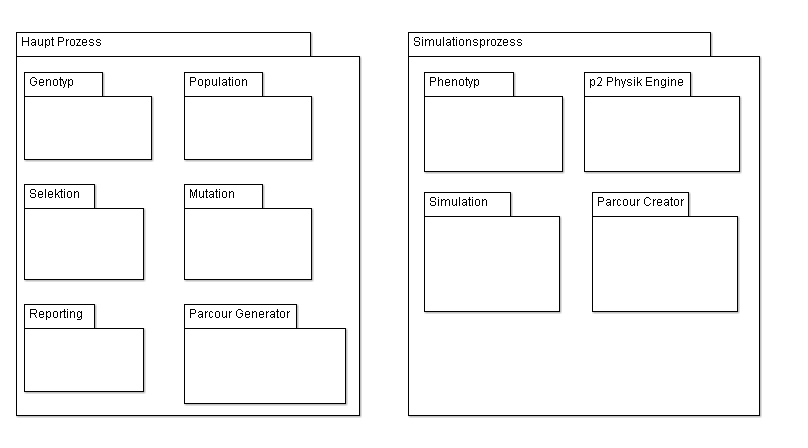
\includegraphics[scale=0.45]{graphics/haupt_simulations_prozess}
      \caption{Haupt- und Simulationsprozess\label{fig:hauptSimuProzesse}}
    \end{figure}
    \begin{figure}[H]
      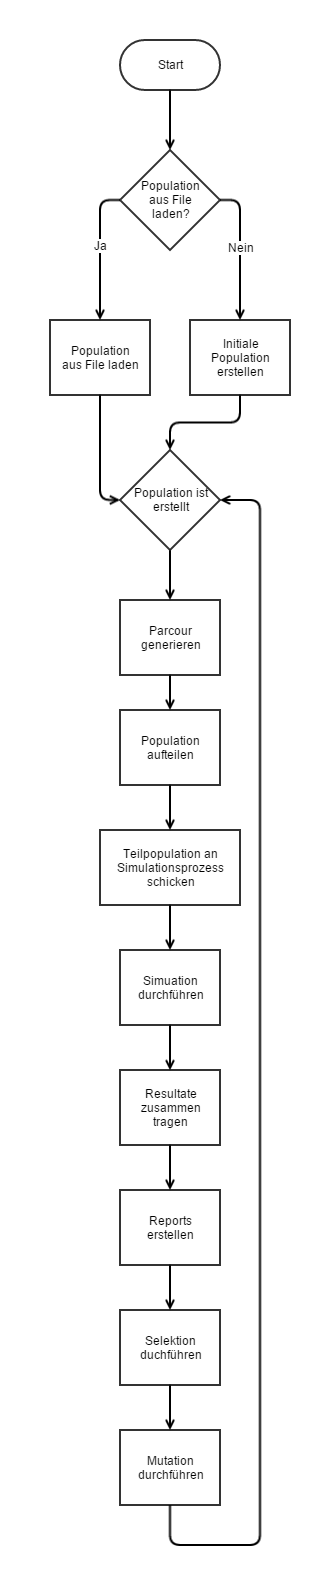
\includegraphics[scale=0.45]{graphics/ablauf}
      \caption{Ablauf der Simulation\label{fig:ablauf}}
    \end{figure}

    \subsection{Initiale Population\label{sec:Initiale Polulation}}

      Als erster Schritt muss eine initiale Population erstellt werden. Die Populationsgrösse kann frei gewhält werden.
      Pro Simulationsprozess können etwa 15 Individuuen flüssig berechnet werden.
      Dies bedeutet das die optimale Populationsgrösse  \( Anzahl(CPU Kerne) * 15 \) beträgt.
      Es werden jeweils Individuen mit 4, 5, 6, 7 und 8 Körperpunkten~\ref{sub:Körper} generiert.
      Die Verantwortliche Klasse in Javascript ist der InitialPopulationGenerator.
      Das Endprodukt dieses Schrittes ist eine Population bestehenden aus den Genotypen der Individuen.

    \subsection{Parcours-Generierung\label{sec:Parcour Generierung}}

      Der Parcours wird zufällig generiert. Am Anfang wird ein einfacher und flacher Parcours generiert.
      Mit zunehmenden Iterationen steigt die Schwierigkeit des Parcours,
      das heisst es werden höhere Steigungen und ein höherer Punkt vorkommen.
      Dazu muss eine Klasse erstellt werden (ParcourGenerator),
      welche mit Hilfe von Obergrenzen von Werten einen Parcours generieren kann.
      Wie unter~\ref{sec:Konfiguration} erwähnt,
      wird je nach Einstellung der Parcours nach jeder Generation neu generiert oder er wird wiederverwendet
      bis ein Abbruchkriterium eintritt.
      Der Parcours wird im ParcourGenerator generiert (Haupt Prozess) und
      von den jeweiligen Worker mit Hilfe vom ParcourCreator in der Physik Engine erstellt.

    \subsection{Simulation}

      Nachdem eine neue Population und ein neuer Parcours erstellt worden ist.
      Muss eine Simulation durchgeführt werden um den Fitnesswert der Individuen zu bestimmen.
      Die Verantwortliche Klasse ist die SimulationWorld.
      Zuerst muss jeder Genotyp zu einem Phenotyp abgebildet werden.
      Anschliessend muss der Parcours aus dem Blueprint erstellt werden.
      Erst dann kann mit der Simulation begonnen werden.
      Die Simulation merkt sich zu jedem Individuum die Position.
      Individuen welche sich während 4 Sekunden kaum bewegt haben,
      werden aus der Simulation entfernt und ihr Fitnesswert wird abgespeichert.
      Die Simulation kann wie unter~\ref{sec:Konfiguration} schon erwähnt, parallelisiert werden.
      Es wird dann jeweils für \( Populationsgrösse / Anzahl Simulationsprozesse \) Individuen eine eigene Simulation erstellt.
      Die Kommunikation zwischen Simulationsprozessen und Hauptprozess erfolgt über asynchrones Messaging.

    \subsection{Reporting\label{subsec:Reporting}}

      Das Reporting-Modul hilft nach einer Simulation alle wichtigen Daten festzuhalten.
      Mithilfe einer Funktion die eine Population als Parameter entgegennimmt,
      werden die Reports erstellt. Es existieren folgende Typen von Reports:
      \begin{itemize}
        \item Fitness Graph Average Report: Enthält Koordinaten um einen Graph über die durchschnittliche Fitness pro Generation zu erstellen.
        \item Fitness Graph Best Report: Enthält Koordinaten um einen Graph über das beste Individuum der Generation zu erstellen.
        \item Genotype Blue Print Report: Enthält pro Generation ein JSON das Informationen über die ganze Population enthält.
        \item Fitness Graph Average Report bp x: Für diesen Typ von Report gibt es jeweils einen für alle Individuen mit Body Points Anzahl x.
        \item Diversity Report: Enthält die Berechnung der Punktstreuung für jeweils eine Generation. Die Punktstreuung berechnet sich wie folgt:
        \begin{itemize}
          \item Erstellung von Vektoren der Genome. Jede Eigenschaft des Genoms wird in einen numerischen Wert konvertiert. \( V_d \)
          \item Alle Vektoren werden summiert.  Die Summe wird als \(V_s\) bezeichnet.
          \item Der Schwerpunktvektor wird gebildet: \( V_s / Anzahl(V_d) = V_{schwer} \)
          \item Von jedem \(V_d\) wird \(V_{schwer}\) subtrahiert  \( V_d - V_{schwer}  = V_{d2} \)
          \item Nun werden alle \(V_{d2}\) normiert, quadriert \( norm{(V_{d2})}^2 = d \)
          \item Abschliessend werden alle \(d\) zusammengezählt und durch \(Anzahl(V_d)\) dividiert. So erhält man ein Mass für die Punktestreuung.
        \end{itemize}
        Ansonsten gleich wie Fitness Graph Average Report.
      \end{itemize}

    \subsection{Selektion\label{sec:Selektion}}

      Als Selektionsstrategie wird tournament-based selection eingesetzt~\ref{par:Turnier}.
      turnierbasierte Selektion hat den Vorteil, dass die Diversität erhalten bleibt,
      bei gleichzeitig guter Selektion der fittesten Individuen.

      \subsubsection{Hypothese Selektionsstrategie\label{sub:Hypothese Selektionsstratgegie}}

        Es wird die Hypothese aufgestellt,
        dass turnierbasierte Selektion die besseren Resultate liefert im Vergleich zu den folgenden Selektionsstrategien: X und Y.
        Um dies zu validieren werden die Selektionsstrategien X und Y implementiert und anschliessend analysiert.
        Ob dies zutrifft wird in Kapitel~\ref{chap:Resulate} diskutiert.

    \subsection{Mutation\label{sec:Mutation}}

      Auf die Selektionsstrategie folgt nun die Mutation der Individuen.
      Bei der Mutation wird über jede Eigenschaft des Individuums iteriert und
      diese wird mit einer bestimmten Wahrscheinlichkeit (PROBABILITY) und um einen bestimmten Wert (STEP) verändert.
      PROBABILITY kann Werte zwischen 0 und 1 annehmen, STEP hat keine Einschränkungen.
      Nachdem für jedes Attribut diese Werte definiert worden sind, kann die Mutation statt finden.
      Grenzen wurden definiert, um nicht gewinnbringende Lösung zu verhindern.
      Solch eine Limit wurde jeweils für die Länge und Breite der Beine aufgestellt.
      Die Position eines Beins wird unter einer zusätzlichen Bedingung mutiert. Falls sich der Körper so verändert hat,
      dass ein Bein ausserhalb des Körper ist, wird die Position zufällig neu bestimmt.
      Die Mutation läuft wie die Simulation parellel ab, das heisst, sie kann von mehreren Kernen in einem Prozessor profitieren.

    \subsection{Wiederholungen}

      Alle Schritte (ausser die Generierung der initialen Population) werden solange ausgeführt,
      bis ein zufriedenstellendes Resultat gefunden wird.

    \subsection{Domänenmodel\label{sub:domMod}}

      Das Domänenmodell beschreibt den Zusammenhang der verschiedenen Klassen und Objekten.
      Abbildung~\ref{fig:mainProcess} beschreibt den Haupt- und Abbildung~\ref{fig:simulationProcess} den Simulationsprozess.
      \begin{figure}[H]
        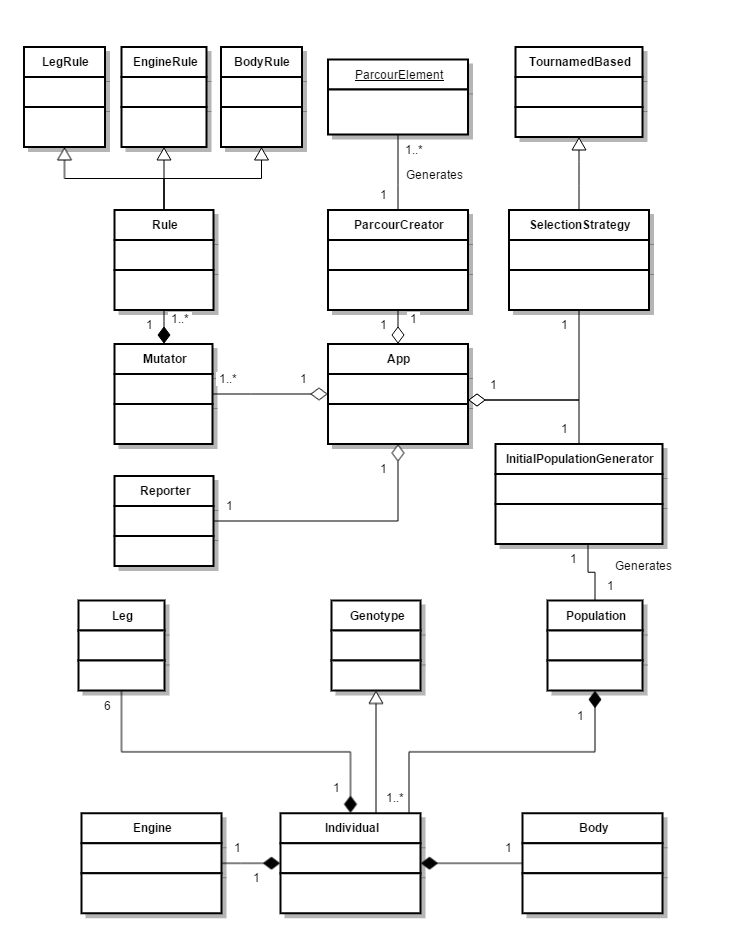
\includegraphics[scale=0.6]{graphics/main_process}
        \caption{Domänen Modell, Hauptprozess\label{fig:mainProcess}}
      \end{figure}
      \begin{figure}[H]
        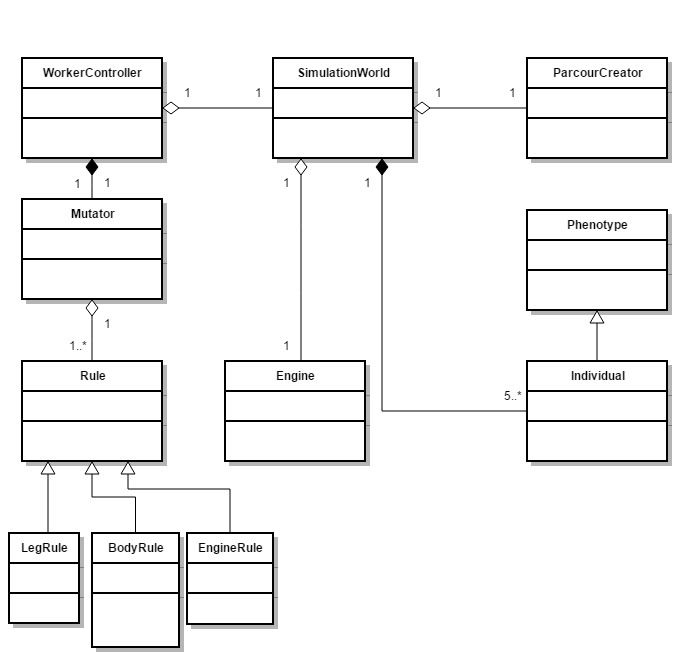
\includegraphics[scale=0.6]{graphics/simulation_process}
        \caption{Domänen Modell, Simulationsprozess\label{fig:simulationProcess}}
      \end{figure}
